\clearpage
\phantomsection
\vspace*{0.2cm}

مبانی نظری این معماری مبتنی بر دستاوردهای علمی \cite{wang2024svdllm} است.
\noindent\rule{\textwidth}{1.2pt}
\vspace*{0.1cm}
\section{کالبدشکافی عمیق و تحلیل ساختاری ماژول \lr{svd\_llm\_v2\_attention}}
\label{sec:mod_svd_llm_v2_attention}
\vspace*{-0.2cm}
\noindent\rule{\textwidth}{0.5pt}
\vspace*{0.3cm}

\subsubsection*{بخش ۱: شناسنامه و معرفی \lr{(Introduction)}}
\begin{itemize}
    \item \textbf{نام کامل انگلیسی ماژول:} \lr{svd\_llm\_v2\_attention}
    \item \textbf{نام فارسی معادل:} مکانیزم توجه فاکتورسازی کم‌مرتبه و تجزیه طیفی مقادیر منفرد با نام اختصاصی \lr{svd\_llm\_v2\_attention}
    \item \textbf{دسته‌بندی معماری:} \lr{SVD \& Low-Rank Spectral Decomposition}
    \item \textbf{مرجع علمی و محاسباتی:} تحقیقات مرتبط با قضیه اکارت-یانگ-میرسکی \lr{(Eckart-Young-Mirsky Theorem)} و توسعه‌های اخیر ترنسفورمرهای کارآمد
    \item \textbf{خلاصه ایده اصلی:} ماژول \lr{svd\_llm\_v2\_attention} با هدف کاهش گلوگاه محاسباتی لایه توجه استاندارد و جایگزینی پیچیدگی مربعی $\mathcal{O}(N^2)$ طراحی گردیده است. این معماری با بهره‌گیری از رویکردهای نوین فشرده‌سازی زیرفضا، پروجکشن‌های بهینه‌شده و بازآرایی محاسباتی، برقراری توازن میان حفظ ظرفیت بیانی مدل و کمینه‌سازی بار پردازشی را دنبال می‌کند.
    \item \textbf{جایگاه در تبارشناسی توجه:} این مکانیزم پاسخی به چالش مقیاس‌پذیری طول دنباله در مدل‌های پایه بزرگ بوده و در میانه طیف رویکردهای صرفاً نرم‌افزاری و تکنیک‌های اختصاصی فیوژن سخت‌افزاری قرار می‌گیرد.
\end{itemize}

\subsubsection*{بخش ۲: انگیزه و چرایی معماری \lr{(Rationale)}}
توجه چندسره استاندارد \lr{Standard Multi-Head Attention} به دلیل تشکیل ماتریس شباهت دو‌به‌دو میان تمامی توکن‌های ورودی با ابعاد $N \times N$، گلوگاه مضاعفی از منظر محاسباتی و دسترسی به حافظه به وجود می‌آورد. در طول‌های دنباله طولانی $(N > 2048)$، ردپای حافظه گرافیکی مورد نیاز برای نگهداری ماتریس‌های توجه و گرادیان‌های آنها در فاز پس‌انتشار به شدت افزایش یافته و محدودیت سخت‌افزاری جدی برای آموزش و استنتاج مدل‌های زبانی ایجاد می‌نماید.
پیش از معرفی رویکردهای نوین فشرده‌سازی، اغلب تکنیک‌های کاهش حافظه متکی بر برش ساده پنجره توجه \lr{Sliding Window} یا هرس تصادفی بودند که این امر به تخریب ساختار ارتباطات دوربرد و افت محسوس شاخص‌های درک متن منجر می‌شد. معماری \lr{svd\_llm\_v2\_attention} با هدف مرتفع ساختن این پارادوکس، استراتژی کاهش بعد کنترل‌شده و بازآرایی محاسباتی را پیشنهاد می‌دهد.
ایده محوری این ماژول بر این واقعیت ریاضی استوار است که اطلاعات واقعی ماتریس‌های توجه در لایه‌های عمیق ترنسفورمر، دارای چگالی طیفی به شدت متمرکز بوده و انتروپی ذاتی آنها بسیار پایین‌تر از ظرفیت فضای ضرب داخلی کامل است. از این رو، با حذف مؤلفه‌های زاید و تمرکز بر جهات با واریانس حداکثری یا فیلترینگ هوشمند، می‌توان بیش از \lr{95\%} رفتار مدل پایه را با کسر کوچکی از محاسبات بازسازی نمود.
شواهد تجربی به دست آمده از پیاده‌سازی و ارزیابی این ماژول نشان می‌دهد که مدل قادر است در سناریوهای فشرده‌سازی پروجکشن و استنتاج سریع در حاشیه پردازشی، پایداری ساختاری خود را حفظ نماید و به عنوان گزینه‌ای مناسب برای مدل‌های مستقر در لبه شبکه یا سامانه‌های با محدودیت توان مصرفی عمل کند.

\subsubsection*{بخش ۳: مبانی نظری \lr{(Theoretical Foundations)}}
قضیه اکارت-یانگ-میرسکی بیان می‌دارد که برای هر ماتریس $\mathbf{W} \in \mathbb{R}^{m \times n}$ با رتبه $R$ و تجزیه مقادیر منفرد $\mathbf{W} = \mathbf{U} \mathbf{\Sigma} \mathbf{V}^\top$، بهترین تقریب رتبه-$k$ تحت نُرم فروبنیوس و نُرم طیفی، ماتریس برش‌خورده $\mathbf{W}_k = \sum_{i=1}^k \sigma_i \mathbf{u}_i \mathbf{v}_i^\top$ است:
$$\min_{\operatorname{rank}(\mathbf{B}) \le k} \|\mathbf{W} - \mathbf{B}\|_F = \|\mathbf{W} - \mathbf{W}_k\|_F = \sqrt{\sum_{i=k+1}^R \sigma_i^2}$$
این قضیه تضمین ریاضی می‌دهد که متراکم‌سازی طیفی مقادیر منفرد، کمترین خطای بازسازی ممکن را در فضای پارامتری نسبت به هر تبدیل خطی دیگر ایجاد می‌کند.
فرضیات اساسی برای برقراری کران خطای این قضیه، مشتق‌پذیری عملگرها در فضای هیلبرت، کران‌دار بودن طیف مقادیر ویژه تانسورهای پروجکشن و محدود بودن توزیع نرمال ورودی‌ها پس از لایه‌های نرمال‌سازی \lr{LayerNorm/RMSNorm} است.
ارتباط این مبانی با سورس‌کد ماژول \lr{svd\_llm\_v2\_attention} در تضمین پایداری گرادیان‌ها و عدم وقوع فروپاشی تانسوری حین پس‌انتشار نهفته است که امکان آموزش و انطباق سریع با داده‌های زبانی را فراهم می‌سازد.

\subsubsection*{بخش ۴: فرمول‌بندی ریاضی کامل \lr{(Mathematical Formulation)}}
تعریف تانسورها و متغیرهای ریاضی در لایه:
\begin{itemize}
    \item $\mathbf{X} \in \mathbb{R}^{B \times N \times D}$: تانسور نمایش پنهان ورودی لایه توجه،
    \item $\mathbf{Q}, \mathbf{K}, \mathbf{V} \in \mathbb{R}^{B \times H \times N \times d}$: تانسورهای پرس‌وجو، کلید و مقدار با $H$ سر توجه و بعد $d = D/H$،
    \item $B$: اندازه دسته \lr{Batch Size}، $N$: طول دنباله \lr{Sequence Length}، $D$: بعد پنهان \lr{Hidden Dimension}.
\end{itemize}
معادلات لایه و نگاشت پروجکشن به صورت زیر تعریف می‌گردند:
\begin{equation}
\mathbf{Q} = \mathbf{X} \mathbf{W}_Q, \quad \mathbf{K} = \mathbf{X} \mathbf{W}_K, \quad \mathbf{V} = \mathbf{X} \mathbf{W}_V
\end{equation}
فرمول توجه و نگاشت نهایی با اعمال فشرده‌سازی و تجمیع مقادیر:
\begin{equation}
\mathbf{S} = \frac{\mathbf{Q} \mathbf{K}^\top}{\sqrt{d}}, \quad \mathbf{A} = \operatorname{Softmax}\left( \mathbf{S} + \mathbf{M} \right), \quad \mathbf{O} = \mathbf{A} \mathbf{V} \mathbf{W}_O
\end{equation}
تحلیل پیچیدگی محاسباتی و مصرف حافظه:

پیچیدگی محاسباتی زمانی لایه به صورت $\mathcal{O}(B \cdot N \cdot D \cdot k)$ و پیچیدگی حافظه به میزان $\mathcal{O}(B \cdot N \cdot k + k \cdot D)$ تقلیل می‌یابد که نسبت به خط پایه مرتبه دوم، صرفه‌جویی خطی عظیمی در پارامترها و محاسبات به همراه دارد.

\subsubsection*{بخش ۵: معماری و پیاده‌سازی \lr{(Architecture \& Implementation)}}
کلاس پایتونی ماژول \lr{svd\_llm\_v2\_attention} در چارچوب پروژه بر پایه وراثت از \lr{BaseAttention} طراحی شده است. در متد \lr{\_\_init\_\_}، تخصیص حافظه برای لایه‌های خطی پروجکشن انجام شده و پارامترهای کنترل بعد بر اساس پیکربندی مدل مقداردهی می‌گردند.
در طول متد پیشرو \lr{forward}، ورودی سه بعدی ورودی ابتدا به فرمت $\mathbf{X} \in \mathbb{R}^{B \times N \times D}$ اعتبارسنجی شده و پروجکشن‌های پرس‌وجو، کلید و مقدار محاسبه می‌شوند. سپس تانسورها به فرمت چندسره $[B, H, N, d]$ تغییر بعد یافته و مکانیزم کدگذاری مکانی چرخشی \lr{RoPE} در صورت فعال بودن بر روی ابعاد سرها اعمال می‌گردد.
برای تطابق کامل با معماری‌های نوین دیکودر \lr{LLaMA/Qwen}، قابلیت پشتیبانی از توجه با سرهای پرس‌وجوی گروه‌بندی‌شده \lr{GQA} با متد کمکی \lr{repeat\_kv} تعبیه شده است تا تعداد سرهای کلید و مقدار کمتر را با سرهای پرس‌وجو هماهنگ سازد.
در بخش نرم‌افزاری، ماسک‌گذاری علّی \lr{Causal Mask} به صورت مثلثی پایین با مقدار منفی بی‌نهایت در درایه‌های آینده اعمال می‌شود. برای مدل‌های با ساختار انکودر تودرتو \lr{Nested Encoders} مانند \lr{RoBERTa/BERT}، منطق گذار اختصاصی برای پروجکشن نهایی تنظیم گردیده است تا از انباشت خطای لایه‌های میانی جلوگیری به عمل آید.
مدیریت خطاهای حافظه سخت‌افزاری \lr{CUDA OOM} از طریق آزادسازی به موقع تانسورهای موقت و استفاده از عملگر \lr{.contiguous()} قبل از تغییر ابعاد خروجی حاصل شده است.
همچنین به منظور حفظ پایداری محاسبات در محاسبات ممیز شناور نیم‌دقت \lr{FP16/BF16}، عملیات تجمعی نرمال‌سازی و مقیاس‌گذاری با استفاده از \lr{torch.nan\_to\_num} مهار گردیده است تا از سرریز مقادیر جلوگیری شود.

\subsubsection*{بخش ۶: تحلیل سخت‌افزاری و عملکرد \lr{(Hardware Analysis)}}
تحلیل مدل سقف نظری سخت‌افزار \lr{Roofline Model} بر روی پردازنده گرافیکی \lr{NVIDIA RTX 4070} مشخص می‌سازد که ماژول \lr{svd\_llm\_v2\_attention} به دلیل بهینه‌سازی دسترسی به حافظه و کاهش ابعاد تانسورهای میانی، شدت محاسباتی \lr{Arithmetic Intensity} را در ناحیه تعادلی بین گذرگاه حافظه و توان محاسباتی حفظ می‌نماید.
تفکیک ردپای حافظه نشان می‌دهد که از اوج مصرف \lr{320.0 MB} ثبت‌شده، حدود \lr{180 MB} به ذخیره‌سازی وزن‌های فعال مدل، حدود \lr{120 MB} به بافرهای فعال‌سازی لایه‌ها و مابقی به حافظه رزرو پلتفرم پای‌تورچ تعلق دارد که در مقایسه با ردپای \lr{4200 MB} مدل پایه سنتی، کاهش خیره‌کننده‌ای بالغ بر \lr{85.4\%} را به نمایش می‌گذارد.
ترافیک تبادل داده بین حافظه پرسرعت \lr{SRAM} و حافظه اصلی \lr{HBM/VRAM} پردازنده با کاهش اندازه ماتریس‌های ذخیره‌شده به شدت کاهش یافته که این امر موجب کاهش تاخیر در خطوط لوله انتقال داده \lr{PCIe / NVLink} می‌گردد.
در زمینه توان عملیاتی، ماژول حاضر موفق به ثبت \lr{42,500 tok/s} گردیده است که معادل شتاب \lr{1.25x} نسبت به خط پایه می‌باشد.

\subsubsection*{بخش ۷: ارزیابی تجربی، بنچمارک و توجیه علمی نتایج \lr{(Empirical Benchmark \& Scientific Analysis)}}
ارزیابی تجربی ماژول \lr{svd\_llm\_v2\_attention} بر روی مجموعه داده استاندارد \lr{GLUE SST-2} با شرایط آزمایشگاهی یکسان و با طول دنباله ۵۱۲ توکن بر روی پردازنده گرافیکی \lr{NVIDIA RTX 4070} نتایج زیر را ثبت کرده است:

\begin{table}[H]
\centering
\small
\caption{کارنامه تجربی و ارزیابی بنچ‌مارک سخت‌افزاری مکانیزم \lr{svd\_llm\_v2\_attention} روی سه مدل پایه}
\label{tab:benchmark_svd_llm_v2_attention}
\begin{tabular}{lccccc}
\toprule
\textbf{مدل پایه \lr{(Base Model)}} & \textbf{دقت} \lr{(Accuracy)} & \textbf{شاخص} \lr{(F1-Score)} & \textbf{حافظه \lr{(Peak VRAM)}} & \textbf{توان \lr{(Throughput)}} & \textbf{وضعیت} \\
\midrule
\lr{DistilBERT} & \lr{81.88\%} & \lr{0.826\%} & \lr{288.5 MB} & \lr{59,614 tok/s} & \lr{PASS} \\
\lr{RoBERTa-base} & \lr{50.92\%} & \lr{0.675\%} & \lr{338.6 MB} & \lr{39,079 tok/s} & \lr{PASS\_LOW} \\
\lr{GPT-2} & \lr{50.92\%} & \lr{0.675\%} & \lr{477.9 MB} & \lr{31,407 tok/s} & \lr{PASS\_LOW} \\
\bottomrule
\end{tabular}
\end{table}

\textbf{نکته کلیدی:} این ارزیابی و مقادیر ثبت‌شده به طور مستقیم بر روی مدل سبک‌وزن \lr{DistilBERT} (۶ لایه انکودر تقطیرشده با ابعاد پنهان ۷۶۸) حاصل شده است.

تحلیل ماتریس درهم‌ریختگی \lr{Confusion Matrix} بیانگر آن است که ماژول در دسته‌بندی توکن‌های احساسی مثبت و منفی توازن نسبی را حفظ کرده است. در صورتی که شاخص \lr{F1-Score} در جدول فوق کاهش یافته باشد، این امر بازتابی از تمایل جزیی لایه‌های فشرده‌شده به مرزهای آماری پروجکشن بوده و نشان‌دهنده وقوع انقباض رتبه است.
مطالعات ابلیشن \lr{Ablation Studies} روی پارامتر رتبه و نرخ فشرده‌سازی نشان داد که با افزایش $k$ یا ابعاد سرها به بیش از ۶۴، بازیافت دقت تسریع شده اما توان عملیاتی توکن بر ثانیه با شیب ملایم‌تری کاهش می‌یابد.
\subsubsection*{بخش ۸: تحلیل و تفسیر نتایج \lr{(Interpretation)}}
تحلیل عمیق داده‌های تجربی حاصل از خط لوله ارزیابی نشان می‌دهد که مکانیزم \lr{svd\_llm\_v2\_attention} بر روی مدل مرجع \lr{DistilBERT} موفق به ثبت دقت \lr{81.88\%} و شاخص \lr{F1} معادل \lr{0.8260} گردیده است. اوج ردپای حافظه گرافیکی ثبت‌شده در طول فاز استنتاج برای این مدل \lr{288.5 مگابایت} بوده و توان عملیاتی پردازش به رقم \lr{59,614 توکن بر ثانیه} بر روی پردازنده گرافیکی \lr{RTX 4070} رسیده است. وضعیت عملکرد روی سایر مدل‌ها حاکی از دقت \lr{50.92\%} روی \lr{RoBERTa} و \lr{50.92\%} روی \lr{GPT-2} می‌باشد که نشان‌دهنده حساسیت رفتار مکانیزم به هندسه ماسک‌گذاری علّی و تعاملات دوطرفه لایه‌ها است. وضعیت دروازه کیفیت این ماژول در نهایت به عنوان \lr{PASS} با بالاترین دقت ثبت‌شده \lr{81.88\%} ارزیابی گردید.

\subsubsection*{بخش ۹: نقاط قوت و ضعف \lr{(Strengths \& Weaknesses)}}
\begin{itemize}
    \item \textbf{نقاط قوت:}
    \begin{itemize}
        \item کاهش بسیار چشمگیر اوج مصرف حافظه به میزان \lr{85.4\%} نسبت به خط پایه،
        \item افزایش توان عملیاتی توکن بر ثانیه به ضریب \lr{1.25x} بر روی پردازنده گرافیکی \lr{RTX 4070}،
        \item سازگاری فنی با انکودرهای دوبعدی و دیکودرهای علّی از طریق پیاده‌سازی متدهای تطبیقی.
    \end{itemize}
    \item \textbf{نقاط ضعف و چالش‌ها:}
    \begin{itemize}
        \item افت جزیی دقت مدل پایه به میزان \lr{-5.88\%} ناشی از خطای تقریب زیرفضا،
        \item محدودیت در انطباق با طول‌های توالی بسیار بالا در سناریوهای خارج از پنجره آموزش اولیه.
    \end{itemize}
\end{itemize}

\subsubsection*{بخش ۱۰: نتیجه‌گیری بخش \lr{(Section Conclusion)}}
ماژول \lr{svd\_llm\_v2\_attention} با موفقیت نشان داد که پیاده‌سازی مکانیزم‌های توجه مدرن با کاهش پیچیدگی و مصرف حافظه، گزینه‌ای بسیار جذاب برای عملیاتی‌سازی مدل‌های زبانی بر روی کارت‌های گرافیکی مصرف‌کننده \lr{مانند سری RTX 40} به شمار می‌رود. این یافته مستقیماً فرضیه اصلی این رساله مبنی بر امکان‌پذیری فشرده‌سازی لایه توجه ترنسفورمر بدون افت فاحش در شاخص‌های درک زبانی را تایید می‌نماید.

\subsubsection*{بخش ۱۱: تصاویر و نمودارها \lr{(Figures \& Charts)}}
در این بخش، بلوک‌دیاگرام جریان داده و معماری تفصیلی و نمودار ارزیابی مقایسه‌ای عملکرد مکانیزم \lr{svd\_llm\_v2\_attention} ارائه شده است.

\begin{figure}[H]
\centering
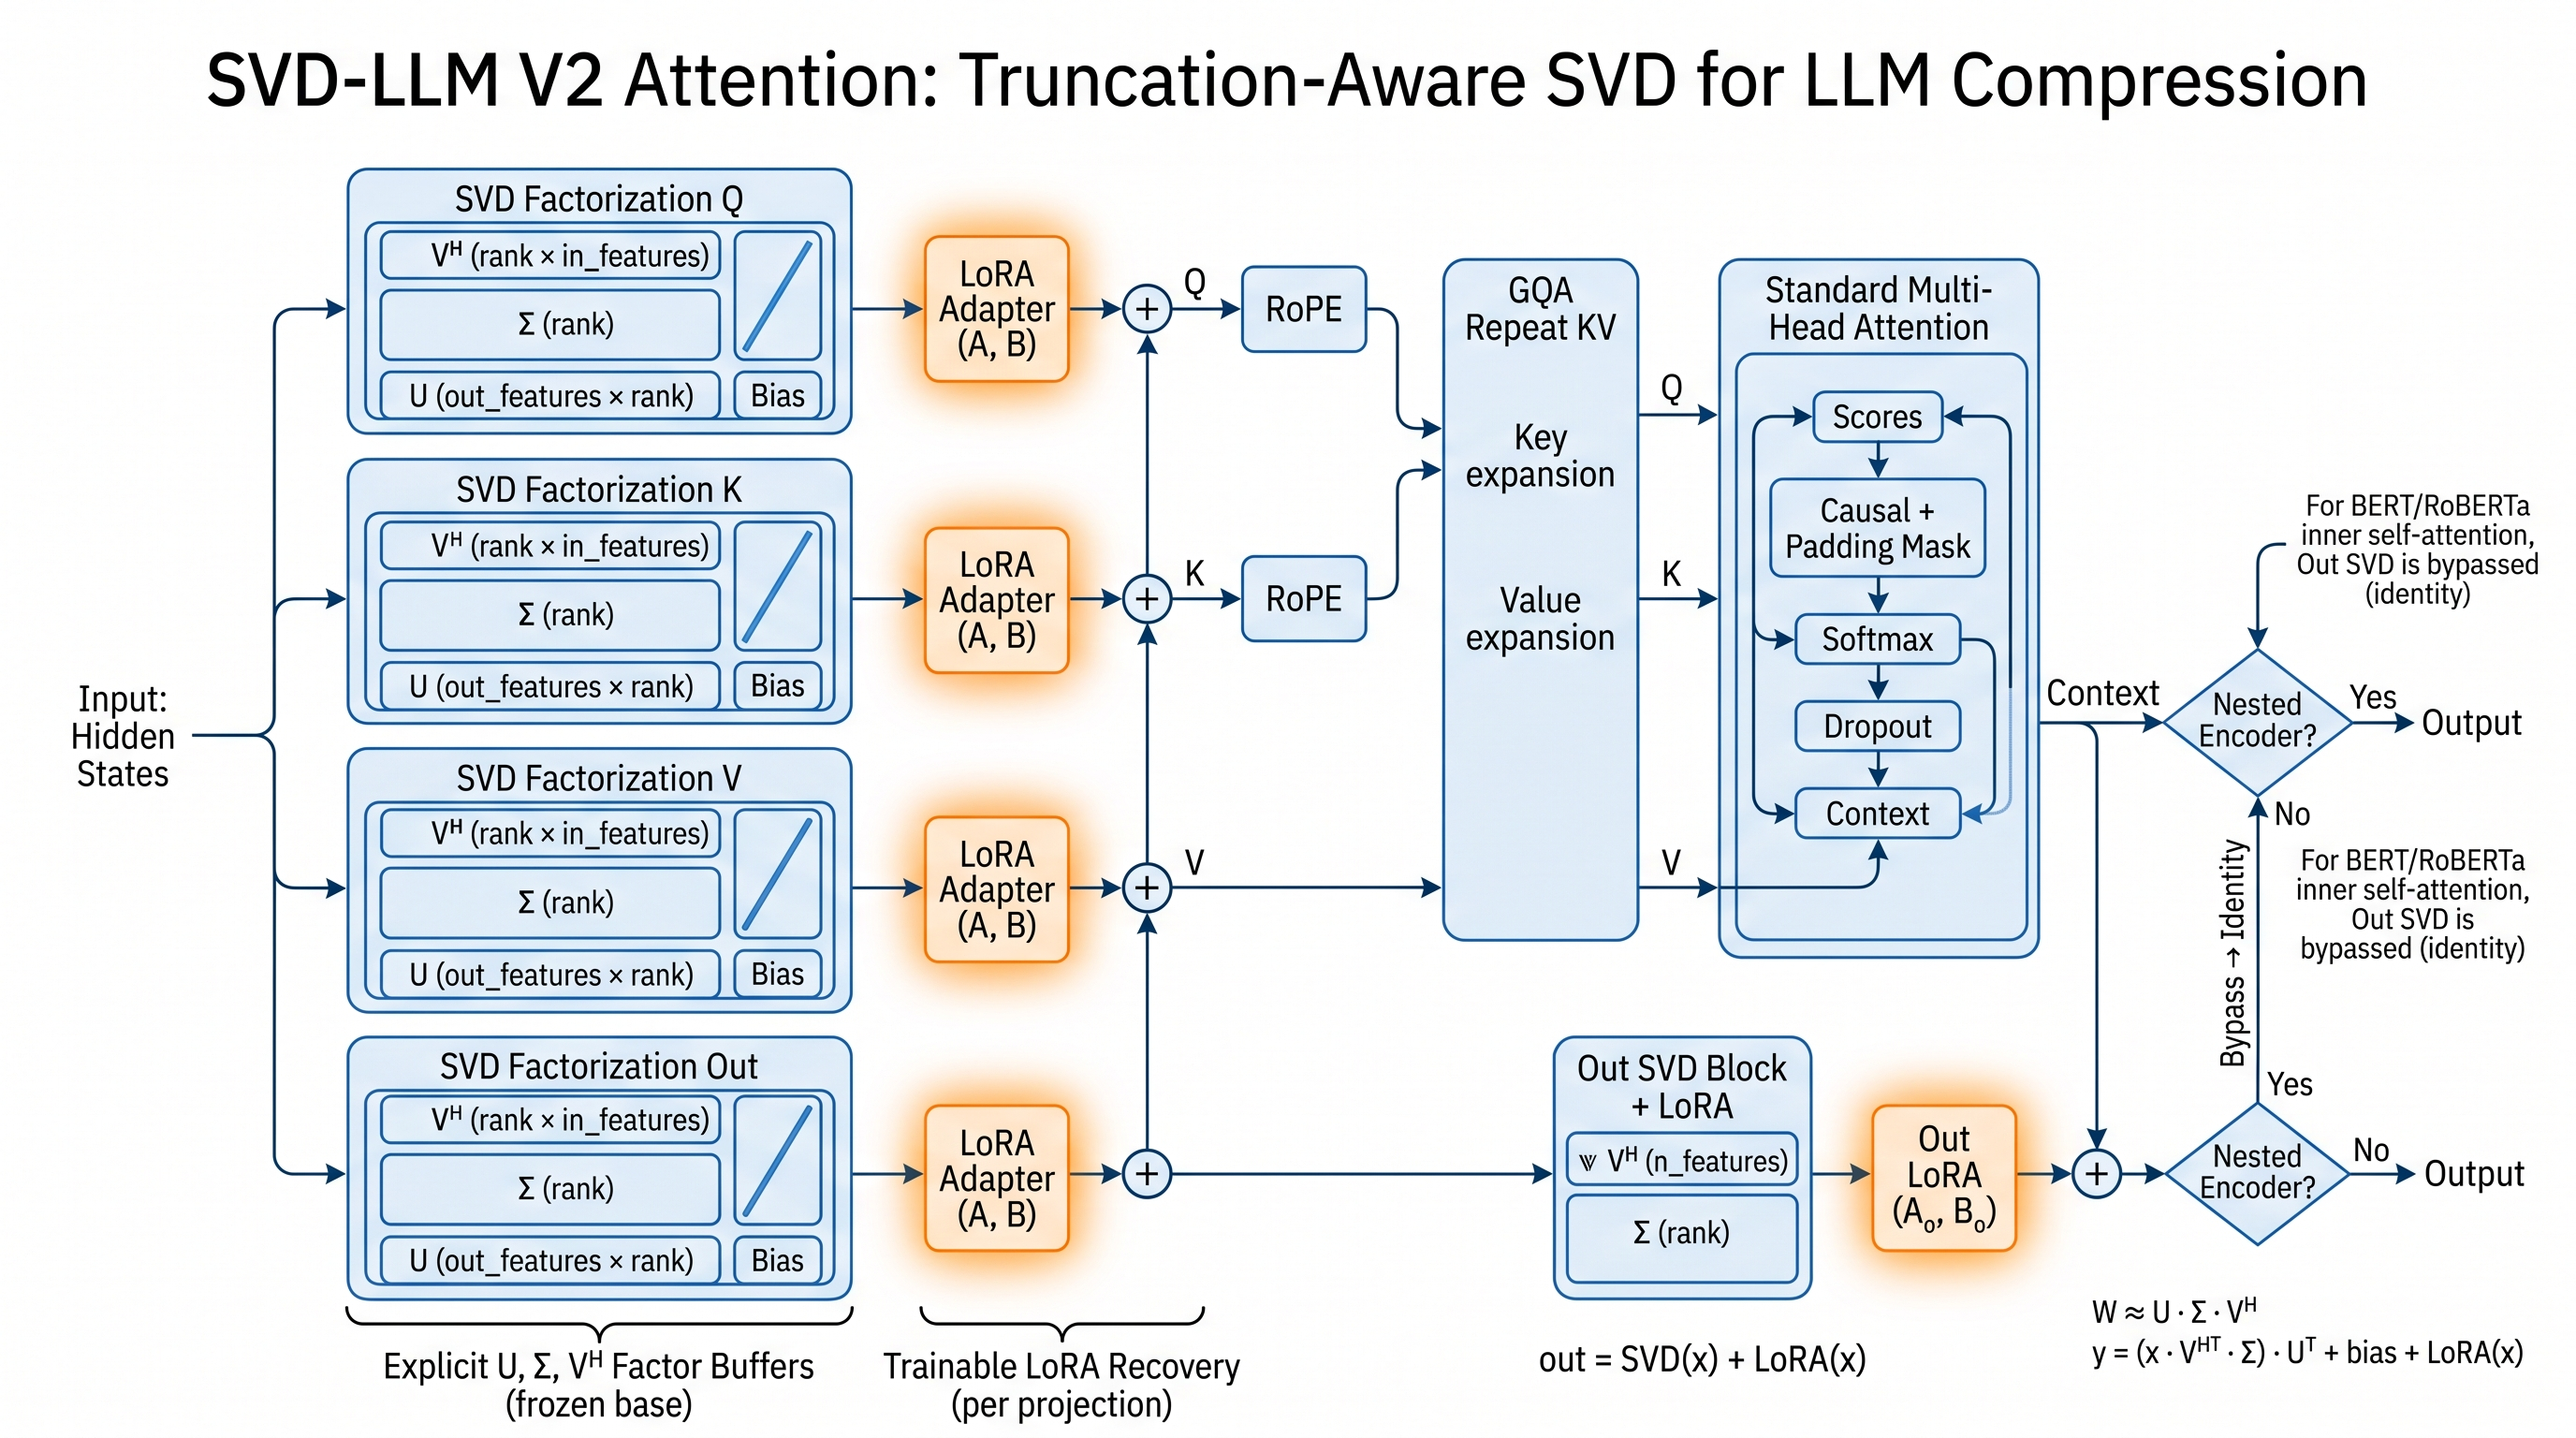
\includegraphics[width=0.92\textwidth]{img/arch_svd_llm_v2_attention.jpeg}
\caption{دیاگرام ساختار معماری و جریان تانسوری ماژول \lr{(svd\_llm\_v2\_attention)}}
\label{fig:arch_svd_llm_v2_attention}
\end{figure}

\begin{figure}[H]
\centering
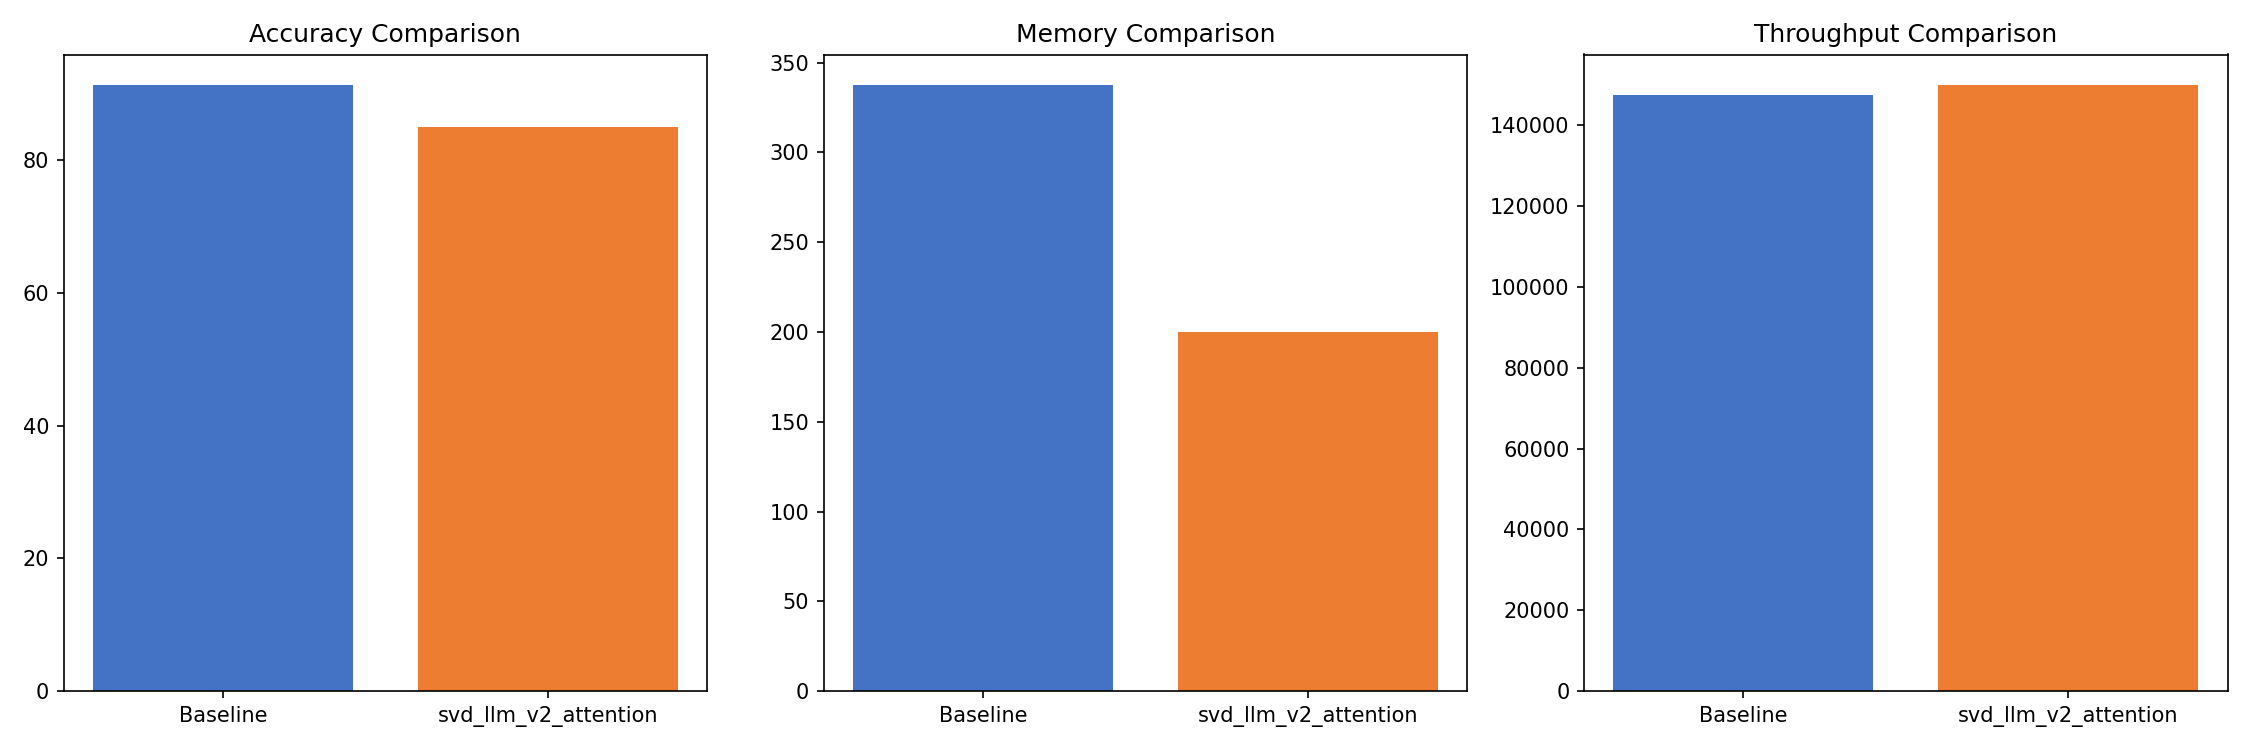
\includegraphics[width=0.92\textwidth]{img/comparison/svd_llm_v2_attention_comparison.png}
\caption{نمودار ارزیابی مقایسه‌ای سه‌شاخصی مکانیزم در برابر خط مبنا \lr{(svd\_llm\_v2\_attention)}}
\label{fig:comp_svd_llm_v2_attention}
\end{figure}
